\chapter{Results and Interpretation}
\label{chap:results}
\shorttitle{\nameref{chap:results}}

This chapter will quantify a difference in the performance of the e-puck2 simulated and physical robot, and Khepera IV simulated robot, showing that the \ac{ros2} interface is appropriately implemented. 
The impact of generalized \ac{ros2} will also be described. 

\section{Comparison of Physical and Simulated E-puck2}

First, the goal is to show whether the \ac{ros2} controller can provide the same results on the physical and simulated e-puck2 robots.
In that regard, a critical sensor camera will be evaluated, and then the whole system will be quantified through \ac{ros2} navigation and mapping controllers.

\subsection{ROS2 Interface for Physical vs. Simulated E-puck2}

There are three benchmarks in which the physical and simulated e-puck2 robots will be compared.
First, the readings from the sensors need to be compared. Most of the sensors of the e-puck2 simulated robot are calibrated before this project has taken place.
Therefore, a quick visual inspection was enough to verify that the sensors have the desired output.
However, this is the first time the camera's resolution is increased to 640x480, producing way more data than before.
In that regard, camera performances are quantified.
Second, to verify whether the whole \ac{ros2} \ac{api} behaves as expected and whether it is compatible with the \ac{ros2} packages, mapping, and navigation will be quantified as well.


\subsection{Camera Performance Comparison}
This benchmark has to compare different \ac{ros2} camera node implementations on the physical e-puck2 robot, at which resolution and \ac{fps} it can operate.
The analysis aims to determine a suitable way to transport the images from Raspberry Pi Zero W and identify bottlenecks.

In terms of compression, the images are transported as raw, \ac{jpeg} compressed and as a Theora compressed video stream\footnote{Description of the Theora technology is available at the official website - \url{https://www.theora.org/}}.
In terms of color encoding \ac{rgb} and \ac{yuv} are tested.
And in terms of nodes separation, the testing node was located on-board or on workstation while communicating to the Raspberry Pi Zero W over Wi-Fi.

In the Table \ref{tab:results:camera_perf}, performances are measured in \ac{fps} and the measurements are given for different camera implementations.

\begin{table}[H]
    \begin{adjustwidth}{-1.5in}{-1.5in} 
    \centering
    \begin{tabular}{|l|c|c|c|}
        \hline
         & 32x24 [\ac{fps} ($ \sigma $)] & 160x120 [\ac{fps} ($ \sigma $)] & 640x480 [\ac{fps} ($ \sigma $)] \\
         \hline
         RAW over Wi-Fi & 13.95 (0.009s) & 10.08 (0.013s) & 1.62 (0.096s) \\
         \hline
         RAW on-board & X & X & 3.80 (0.064s) \\
        \hline
        JPEG over Wi-Fi & X & X & 2.97 (0.105s) \\
        \hline
        JPEG over Wi-Fi with white-noise & X & X & 0.95 (0.998s) \\
        \hline
        JPEG on-board & X & X & 2.10 (0.016s) \\
        \hline
        RAW on-board without YUV42RGB & X & X & 5.04 (0.037s) \\
        \hline
        Theora over Wi-Fi & X & X & 1.25 (0.054s) \\
        \hline
        Theora on-board & X & X & 1.03 (0.026s) \\
        \hline
        Custom over Wi-Fi & 10.079 (0.073s) & 9.981 (0.076s) & 9.904 (0.079s) \\
        \hline
    \end{tabular}
    \end{adjustwidth}
    
    \caption{\ac{fps} measurements in different configurations within \ac{ros2} environment}
    \label{tab:results:camera_perf}
\end{table}

Please note that the experiments are done under the following conditions:
\begin{itemize}
    \item Package \texttt{v4l2\_camera} is used to read and transport images. The package works as following:
        \begin{itemize}
            \item the images are read directly from memory using \texttt{mmap()} in YUV422\_YUY2 format (native camera format),
            \item the images are converted to \ac{rgb} color encoding using \texttt{cv\_bridge} package and
            \item the images are transported using \texttt{image\_transport}, \texttt{image\_transport\_plugins} (equipped with \texttt{compressed\_image\_transport} and \texttt{theora\_image\_transport}) with default configuration,
            \item the package is alternated to accommodate image resize for this experiment and the image resizing is done just before YUV422\_YUY2 to \ac{rgb} conversion and
            \item the package is implemented in C++ with attention to memory management (the image is cloned only when necessary).
        \end{itemize}
    \item Camera is configured to 15 \ac{fps}.
    \item \ac{fps} measurements are done using \texttt{ros2 topic hz}.
    \item The Wi-Fi network performance measurements are performed using \texttt{iperf3} and the following results acquired:
        \begin{itemize}
            \item 16.4 Mbits/sec for transfer from \ac{pc} to Raspberry Pi Zero W and
            \item 13.8 Mbits/sec for transfer from Raspberry Pi Zero W to \ac{pc}.
        \end{itemize}
    \item White noise is simulated by putting finger on the camera.
    The assumption is that the low light condition produces a lot of white noise. 
\end{itemize}

Measured data transfer between Raspberry Pi Zero W and \ac{pc} during the publishing of the raw images is 12.8Mb/s, which is quite close speed measured using with \texttt{iperf3}.
Since every image is sent in \ac{rgb} format that means 7Mbits per image ($ 8 \times \frac{ 3 \times 640 \times 480 }{1024 \times 1024}$), or at 1.62 \ac{fps} it is 11.4Mbits/s.
Therefore, by sending raw images, we most probably encounter limitations of the Wi-Fi network.

In all other methods that require compression (\ac{jpeg} or Theora), the \ac{cpu} on Raspberry Pi Zero W was hitting 100\% of the load.
Therefore, in those cases, the \ac{cpu} is the bottleneck.

Compare achieved \ac{fps} while using \ac{jpeg} compressed images on-board and over Wi-Fi. 
It may look strange that a slightly higher \ac{fps} is achieved with the images that are transferred over the network. 
But note that Raspberry Pi Zero W has a very slow \ac{cpu} and that the tool used to measure performance has to allocate a certain amount of \ac{cpu} time.
Since the network is not the bottleneck here, but \ac{cpu}, the effect of another process using \ac{cpu} is noticeable.

\begin{figure}[H]
\centering
\begin{subfigure}{.8\textwidth}
  \centering
  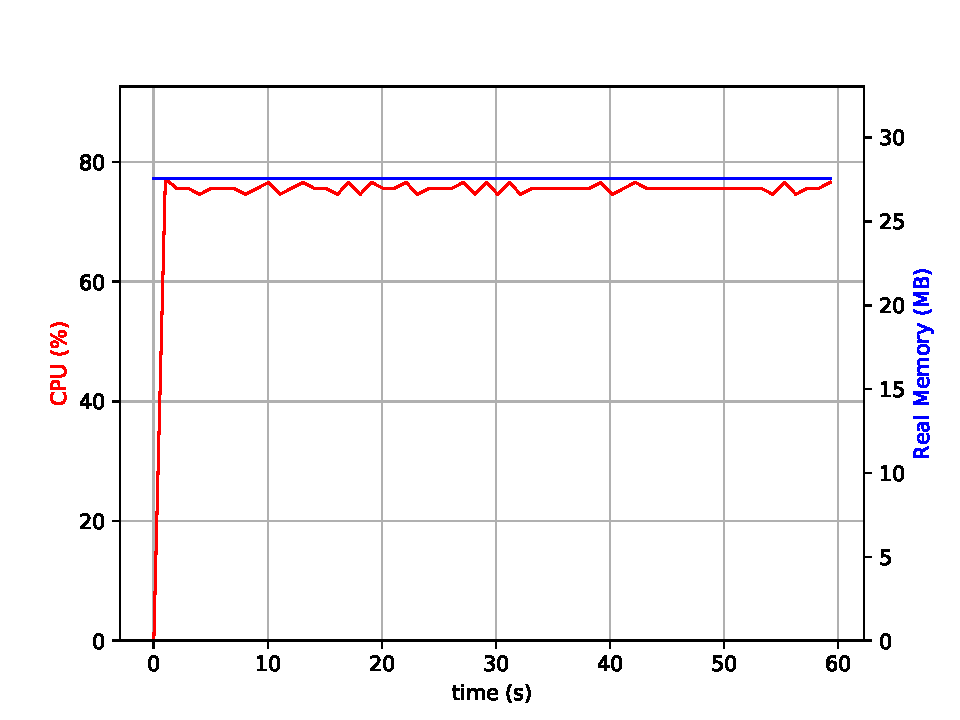
\includegraphics[width=\linewidth]{results/figures/camera_raw_cpu}
  \caption{\ac{cpu} usage while publishing raw \ac{rgb} images}
  \label{fig:results:camera_load:raw_cpu}
\end{subfigure}
\begin{subfigure}{.8\textwidth}
  \centering
  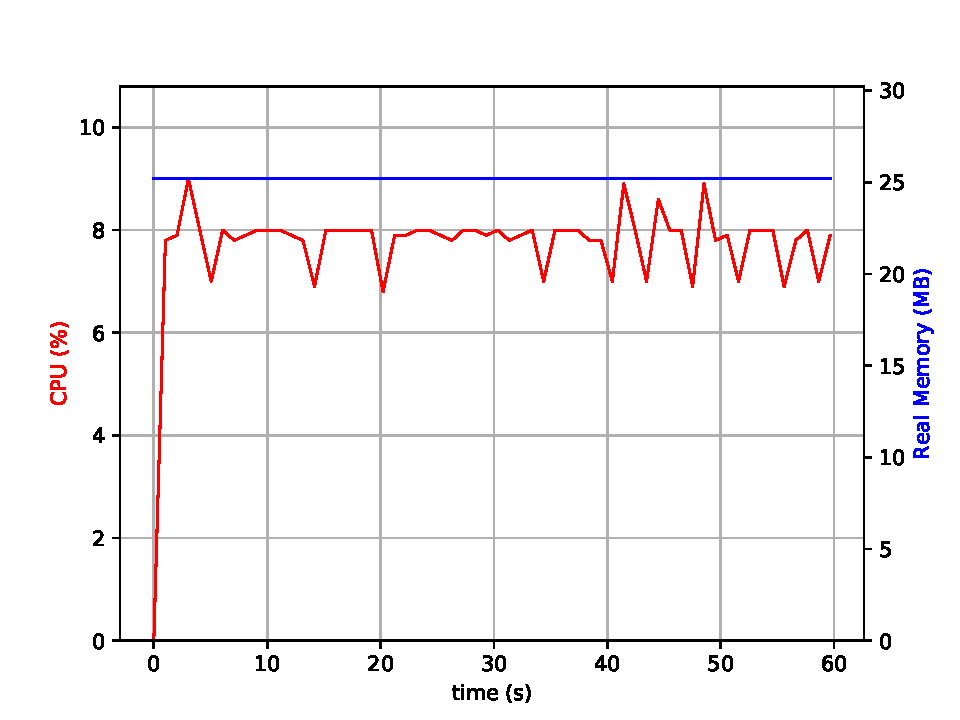
\includegraphics[width=\linewidth]{results/figures/camera_jpeg_gpu.pdf}
  \caption{\ac{cpu} usage while publishing \ac{jpeg} compressed images compressed on \ac{gpu}}
  \label{fig:results:camera_load:jpeg_gpu}
\end{subfigure}
\caption[Comparison of \ac{cpu} usage for two transfer modes, raw \ac{rgb} and \ac{jpeg} compressed on \ac{gpu}]{Comparison of \ac{cpu} usage for two transfer modes, raw \ac{rgb} (named as ``RAW over Wi-Fi" in Table \ref{tab:results:camera_perf}) and \ac{jpeg} compressed on \ac{gpu} (named as ``Custom over Wi-Fi" in Table \ref{tab:results:camera_perf})}
\label{fig:results:camera_load}
\end{figure}

In Fig. \ref{fig:results:camera_load} \ac{cpu} load of two modes are compared.
It shows that even though there is no compression involve, just image publishing, the images are too big for Raspberry Pi Zero W to be transmitted, and the process allocates a lot of \ac{cpu} time.
In contrast, there the images compressed with \ac{gpu} are the small and cumbersome process of compression is offloaded to \ac{gpu}, leaving \ac{cpu} with a minimal load.

\subsection{Performance Comparison in Mapping}
In Section \ref{sec:demos:mapping} a custom \ac{ros2} node for mapping is described. Here, it will be used by e-puck2 physical and simulated robot for performance comparison. In that purpose a physical map is created, as well as, its digital copy in Webots (see Fig. \ref{fig:results:camera_load}).

\begin{figure}[H]
\centering
\begin{subfigure}{.452\textwidth}
  \centering
  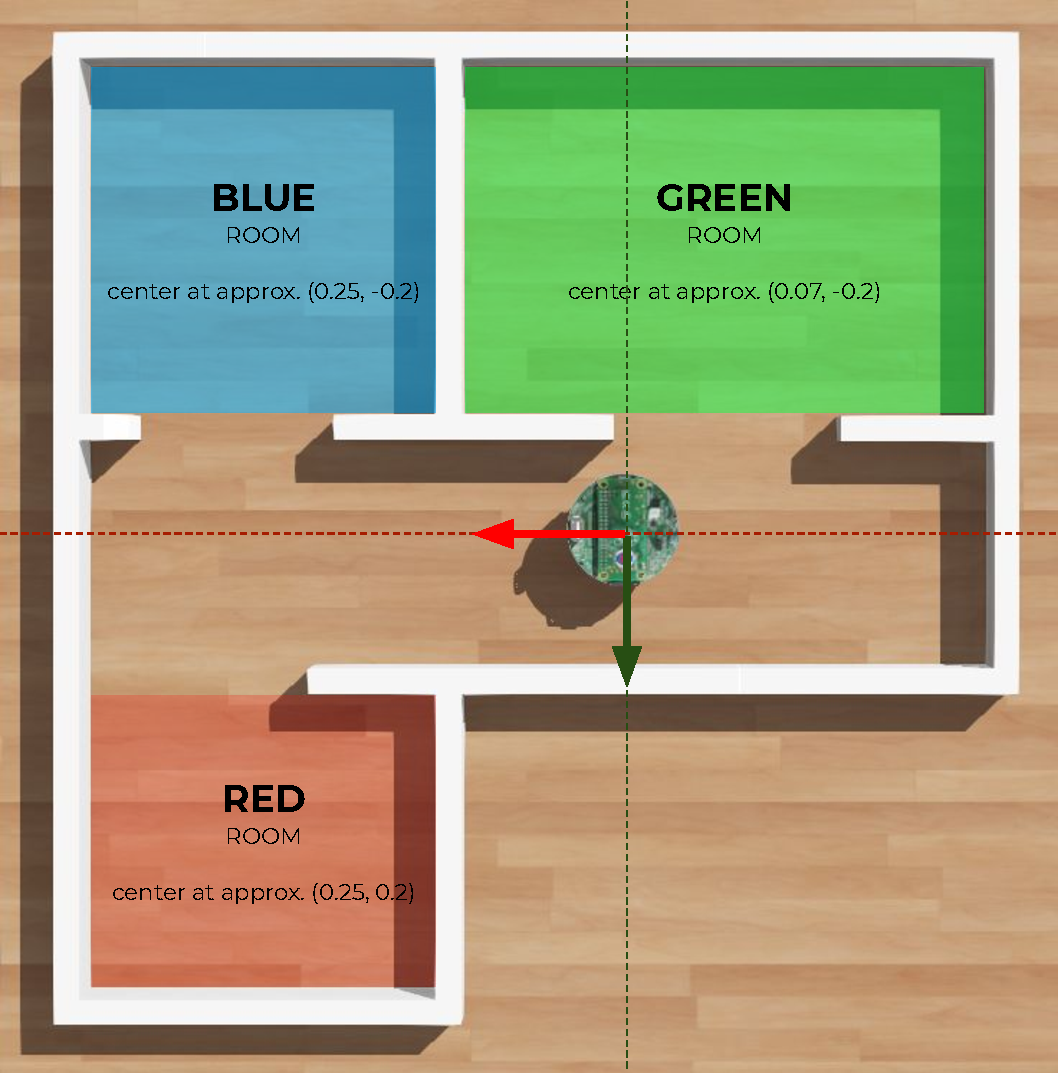
\includegraphics[width=0.97\linewidth]{results/figures/map_webots}
  \caption{Webots map}
  \label{fig:results:map:map_webots}
\end{subfigure}%
\begin{subfigure}{.448\textwidth}
  \centering
  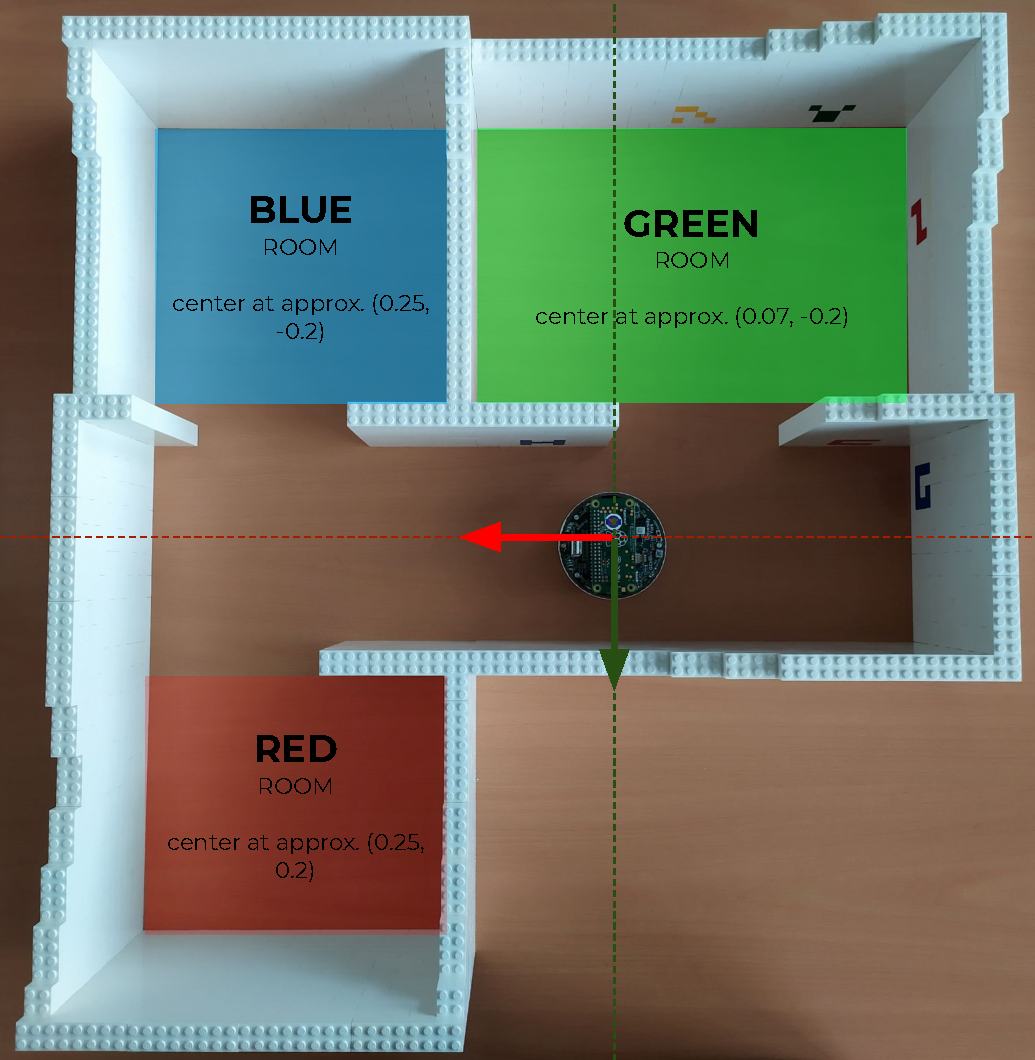
\includegraphics[width=0.97\linewidth]{results/figures/map_real_world}
  \caption{Real-world map}
  \label{fig:results:map:map_real_world}
\end{subfigure}
\caption[Webots map used for the mapping benchmark]{Webots and physical map used for the mapping benchmark with room names and coordinate systems marked}
\label{fig:results:camera_load}
\end{figure}


\subsection{Performance Comparison in Navigation}

\section{\ac{ros2} Interface for E-puck2 vs Khepera IV}
\subsection{Performance Comparison in Mapping}
\subsection{Performance Comparison in Navigation}

\section{Benefits of Generalized \ac{ros2} Interface for Webots}
\subsection{Simplification of E-puck2 Driver}
\subsection{Khepera IV Driver Analysis}
\subsection{Going Beyond Khepera IV and E-puck2}
\subsubsection{TurtleBot3 Burger Robot}
\subsubsection{TIAGo Robot}
